\chapter{Reinforcement Learning and Deep Neural Networks}
\label{ch:reinforcement_learning}


\begin{remark}{Outline}
This chapter introduces the research field of Reinforcement Learning (RL) and presents how its algorithms can successfully be combined with neural networks. The successful marriage between RL and deep neural networks comes with the name of Deep Reinforcement Learning (DRL) and builds on top of research that dates back to a time when training neural networks was not the common practice it is nowadays. We start by providing a general introduction to the field of RL in Sec. \ref{sec:rl_introduction} where we describe the main objectives of this machine learning paradigm and see how it differs from the supervised learning setting that we have described in the previous chapter. We then present the mathematical framework that underpins the development of RL algorithms in Sec. \ref{sec:mdps}, \ref{sec:goals_and_returns} and \ref{sec:value_functions}. In Sec. \ref{sec:learning_value_functions} and Sec. \ref{sec:function_approximators} we describe how one can create RL algorithms and why it is desirable to integrate the resulting algorithms with neural networks. In Sec. \ref{sec:deep_reinforcement_learning} we describe the field of DRL and introduce some of the most popular techniques that have been proposed over the years. This chapter ends with Sec. \ref{sec:challenges} where we discuss one of the main challenges that currently characterizes DRL and that has served as inspiration for the research that will be presented in Chapters \ref{ch:dqv_family_of_algorithms} and \ref{ch:dqn_transfer} of this dissertation.

\end{remark}

\section{Introduction}
\label{sec:rl_introduction}
In Chapter \ref{ch:supervised_learning}, we have described Supervised Learning (SL), a machine learning framework that aims at constructing models which can answer statistical questions about data coming in the form of input-output pairs. When these models are built successfully, it is possible to use them to make predictions about the behavior of new unseen data. Training SL models is a process which from some perspective is very static. Datasets are divided into training, validation, and testing sets, and besides providing a model with a large set of samples drawn from these datasets, there is no real interaction between the learning algorithm and the data that drives the learning process. In Reinforcement Learning (RL), this changes drastically. The goal is not to learn a mapping between a set of fixed input samples and their respective targets, but to train an algorithm that learns how to interact with an environment. RL is, therefore, a much more dynamic learning paradigm, where the concept of time is omnipresent and is critical for the development of algorithms that not only need to solve a specific problem, but additionally, also have to be able to adapt themselves while training progresses.

In RL, a learning algorithm is usually called the \textcolor{RoyalBlue}{agent}, and it can come in numerous forms: it can range from being a self-driving car that needs to learn how to drive; to a recommendation system whose goal is to propose products to users navigating the web. More generally, we define an RL agent as any system that, given a specific situation, has to choose which action to perform. However, there is one more additional component that makes RL the challenging machine learning setting it is.
It is not enough for an agent to just learn how to interact with the environment, it is even more desirable for it to learn an interaction which can be defined as "intelligent". Going back to the self-driving car example, an "intelligent" agent would not only be a car that can drive autonomously, but a car that is also able to do this while complying with the driving code. Because of this concept of learning how to make (intelligent) decisions while interacting, the problems tackled by RL algorithms are also reffered to as optimal decision making problems, which are also the target of research fields other than machine learning, such as control theory. Interestingly, both worlds try to solve the same set of problems, one by tackling them through algorithms that are denoted as "intelligent", while the other through the development of algorithms that are "optimal." Throughout this dissertation, we will not make a clear distinction between these two worlds and will assume that algorithms yielding intelligent behaviors also result in optimal behaviors. Nevertheless, we encourage the reader that has finished reading this chapter to assess whether acting optimally necessarily coincides with acting intelligently.

\section{Markov Decision Processes}
\label{sec:mdps}

Before starting to develop RL algorithms for sequential decision making problems, we formulate the problem within the mathematical framework of Markov Decision Processes (MDPs) \cite{puterman1990markov,puterman2014markov}. Throughout this dissertation, we will characterize MDPs, and the resulting RL concepts, by using the mathematical notation that was used by \citet{sutton2018reinforcement} in their seminal book about RL, although it is worth noting that within the literature, different formulations can be found for expressing the same kind of concepts \cite{bertsekas1995neuro,busoniu2010reinforcement,bertsekas2000dynamic,bertsekas2019reinforcement}.

We start by introducing the following elements:
\begin{itemize}
	\item A set of possible states $\mathcal{S}$, that can be visited by an agent while it is interacting with the MDP, where $s_t \in \mathcal{S}$ denotes the state being visited at time-step $t$.
	\item A set of possible actions $\mathcal{A}$ that are available to the agent when it is in a certain state, where $a_t \in \mathcal{A}(s_t)$ denotes the action that is performed by the agent in state $s$ at time-step $t$.
\item A transition function $\mathcal{P}:\mathcal{S}\times\mathcal{A}\times\mathcal{S}\rightarrow [0,1]$ that defines the probability for an agent to visit state $s_{t+1}$, based on its current state and the action which will be performed thereafter.
\item A reward function $\Re:\mathcal{S}\times\mathcal{A}\times\mathcal{S}\rightarrow \mathbb{R}$ which returns a reward signal $r_{t}$ when an agent performs action $a_t$ in state $s_t$ and transits to $s_{t+1}$.
\item A discount factor denoted as $\gamma \in [0,1]$ (explained in Section \ref{sec:goals_and_returns}).

\end{itemize}

Based on these concepts a MDP is defined by the following tuple $\langle\mathcal{S}, \mathcal{A}, \mathcal{P}, \Re, \gamma\rangle$ and is also commonly denoted in the RL literature as the \textcolor{RoyalBlue}{environment}. The way the agent interacts with this environment is given by its \textcolor{RoyalBlue}{policy} $\pi$, defined as a probability distribution over $a \in \mathcal{A}(s)$ for each $s \in \mathcal{S}$:
\begin{equation}
	\pi(a|s) = \text{Pr}\; \{a_t = a | s_t = s\}, \; \text{for all}\; s \in \mathcal{S}\; \text{and}\; a\ \in \mathcal{A}. 
\end{equation}
Policies can be deterministic if $\forall s: \pi(a|s) = 1$ for exactly one $a\in \mathcal{A}(s)$ and $\pi(b|s) = 0$ for all $b\in \mathcal{A}(s)\setminus\{a\}$. A policy is also stationary if it does not change over time.

%or stationary, in both cases we can define them as follows:
%\begin{definition}
%	A policy $\pi:\mathcal{S}\rightarrow\mathcal{A}$ is a mapping from states to actions. 
%\end{definition}

The elements of the MDP allow us to properly model the dynamics of an agent interacting with its environment, an interaction which can be summarized as follows: at each time-step $t$ the environment provides the agent with a certain state $s_t$, the agent then performs action $a_t$ which results into the reward signal $r_{t}$. After performing such action the agent will enter into a new state $s_{t+1}$. This continuous interaction with the environment is also known as the Reinforcement Learning loop, and can technically be infinite. However, this is never the case in practice, as an agent will eventually visit a state (denoted as terminal) that only transits to itself, which will therefore stop the agent-environment interaction. We visually represent the Reinforcement Learning loop in Fig. \ref{fig:rl_loop}.

\begin{figure}[htb!]
	\centering
	\tikzset{
  frame/.style={
    rectangle, draw,
    text width=6em, text centered,
    minimum height=4em,drop shadow,fill=white,
    rounded corners,
  },
  line/.style={
    draw, -{Latex},rounded corners=3mm,
  }
}

\begin{tikzpicture}[font=\small\sffamily\bfseries,very thick,node distance = 4cm]
\node [frame] (agent) {Agent};
\node [frame, below=1.2cm of agent] (environment) {Environment};
\draw[line] (agent.0) -- ++ (1.5,0) |- (environment.0) 
node[right,pos=0.25,align=left] {action\\ $a_t$};
\coordinate[left=8mm of environment] (P);
\draw[thin,dashed] (P|-environment.north) -- (P|-environment.south);
\draw[line] (environment.200) -- (P |- environment.200)
node[midway,above]{$s_{t+1}$};
\draw[line,thick] (environment.160) -- (P |- environment.160)
node[midway,above]{$r_{t+1}$};
\draw[line] (P |- environment.200) -- ++ (-1.4,0) |- (agent.160)
node[left, pos=0.25, align=right] {state\\ $s_t$};
\draw[line,thick] (P |- environment.160) -- ++ (-0.8,0) |- (agent.200)
node[right,pos=0.25,align=left] {reward\\ $r_t$};
\end{tikzpicture}


\caption{A visual representation of how an agent interacts with an environment as modeled by a Markov decision process. Figure inspired by page 48 of the \citet{sutton2018reinforcement} textbook.}
  \label{fig:rl_loop}
\end{figure}

Each interaction of the agent with the environment is defined as an \textcolor{RoyalBlue}{episode}, which consists of one or several trajectories $\tau$ that come in the form of the following sequence:
\begin{align}
	\langle(s_t,a_t,r_t,s_{t+1})\rangle,t=0,\ldots,T-1
\end{align}
where $T$ is a random variable representing the length of the episode.

A key property of the environment is that it fulfills the Markov property which is defined as follows:
\begin{definition}
	A discrete stochastic process is Markovian if the conditional distribution of the next state of the process only depends from the current state of the process.
\end{definition}
This implies that the only information that is necessary for predicting to which state an agent will step next are $s_t$ and $a_t$, a concept which can be expressed formally as:
\begin{align}
	p(s_{t+1}|s_t, a_t, s_{t-1}, a_{t-1}, \ldots) = p(s_{t+1} | s_t, a_t).
\end{align}
Interestingly, the same property is also assumed for the reward that the agent will get, meaning that the reward that an agent obtains is only determined by its previous action, and not by the history of all previously taken actions, as defined by:
\begin{align}
	p(r_t| s_t, a_t, \ldots, s_1, a_1) = p(r_t|s_t,a_t).
\end{align}


\section{Goals and Returns}
\label{sec:goals_and_returns}
So far, we have defined all the elements that model an agent's interaction with an environment while introducing some of its fundamental properties. However, we do not yet know what the purpose of this interaction is. In RL, an agent's goal is defined with respect to the reward signal $r_t$ that is returned by the reward function $\Re$ and is very straightforward: maximizing the total amount of reward it receives while interacting with the environment. In the simplest case, we can define this as:
\begin{align}
	G_t = r_t + r_{t+1} + r_{t+2} + \ldots + r_{T}.
\label{eq:goal}
\end{align}
While simple and intuitive, this formulation has one major drawback: it treats each reward signal equally as it does not distinguish rewards that are obtained in the near future, $r_t$, from the ones that will be obtained in the more distant future, $r_{T-1}$. To deal with this issue, we need an additional concept known as \textcolor{RoyalBlue}{discounting}, and that is governed by the discount rate parameter $\gamma$, also known as the discount factor. $\gamma$ allows us to weight the different reward signals based on how close or distant in the future these rewards are received by the agent. By introducing $\gamma$ in Eq. \ref{eq:goal} we can now define the expected discounted return as:
\begin{equation}
	\begin{split}
	G_t & = r_t+\gamma r_{t+1} + \gamma^{2} r_{t+2} + ... \\
	    & = \sum_{k=0}^{\infty}\gamma^{k} r_{t+k}.
	\end{split}
\label{eq:discounted_return}
\end{equation}
The role of $\gamma$ can be interpreted as follows: a reward obtained $k$ time steps in the future is only worth $\gamma^{k-1}$ times what it would be worth if received immediately. It is easy to see how different $\gamma$ values can result in different agent's behaviors. If $\gamma=0$ an agent will only take into account immediate rewards, therefore aiming to maximize $r_{t+1}$ only and resulting into having a "myopic" behavior. If $\gamma$ approaches $1$ the agent will become more "far-sighted", it will take future rewards into account more strongly and will therefore increase its chances of accessing rewards that will result into a higher cumulative return. 
Please note that by defining $\gamma < 1$, we can make the infinite sum presented in Eq. \ref{eq:discounted_return} finite as long as the rewards $r_k$ are bounded.

While the role of $\gamma$ is often taken for granted within the RL literature, it is worth noting that as mentioned by \citet{hessel2019inductive} and \citet{schmidhuber2019reinforcement}, $\gamma$ is an artificial concept that is not present in fields such as traditional control theory or engineering. This is because $\gamma$ corresponds to a concept that does not exist in the real world and that in practice distorts the actual value of $r_t$ in an exponentially shrinking fashion. Even if it is considered standard practice to include a discount factor in the development of RL algorithms, it is worth noting that making $\gamma$ part of the RL framework corresponds to including a form of "inductive bias" within the resulting algorithms. It is common knowledge that low discount factors result in poor performance and that it is therefore beneficial to set $\gamma$ as close to $1$, yet choosing an appropriate $\gamma$ parameter can be more challenging than expected, especially when RL algorithms are combined with function approximators. For example, \citet{wiering2009qv} show that different algorithms prefer different discount factors, while \citet{franccois2015discount} show the benefits of initially starting with a low discount factor which gradually gets increased while training progresses. Finally, \citet{vanseijen2019using} introduce a method that allows the use of low discount factors for approximate RL algorithms while at the same time highlighting that the common perception of the role of $\gamma$ might need revision from the RL community. We discuss an alternative perspective to solving RL problems that does not involve the role of $\gamma$ in Appendix \ref{ch:appendixupsidedown}.             

\section{Value Functions}
\label{sec:value_functions}
We are now ready to introduce the arguably most important concept underlying many RL algorithms: the concept of \textcolor{RoyalBlue}{value}. We can define the value of a state $s$, as well as the value of a specific policy $\pi$ or of a particular action $a$, anyhow, independently from what we are considering, the notion of value is always directly linked to the concept of expected discounted return defined in Eq. \ref{eq:discounted_return}. Given an MDP and a policy $\pi$, we can determine the value of a state $s$ as a function $V^\pi:\mathcal{S}\rightarrow\mathbb{R}$ that measures the expected return that the agent will receive when starting in $s$ and following $\pi$ thereafter. 
\begin{align}
    V^{\pi}(s)=\mathds{E}\bigg[\sum_{k=0}^{\infty}\gamma^{k}r_{t+k}\bigg| s_t = s, \pi \bigg].
    \label{eq:state_value_function}
\end{align}
$V^{\pi}(s)$ is also known as the state-value function and intuitively tells us how good or how bad it is for an agent to be in a certain state. While this function is only conditioned on the state that is being visited by the agent, we can also condition it on the actions that the agent takes. By doing so we will quantify how good or bad it is for the agent to take a certain action $a$ in a certain state. This function $Q^\pi:\mathcal{S}\times \mathcal{A} \rightarrow\mathbb{R}$ comes with the name of state-action value function and is defined as follows:
\begin{align}
     	Q^{\pi}(s,a)=\mathds{E}\bigg[\sum_{k=0}^{\infty}\gamma^{k}r_{t+k} \bigg| s_t = s, a_t=a, \pi\bigg].
\end{align}
Both value functions are very powerful as they allow to characterize an agent's behavior by quantitatively assessing its interaction with the environment. They can be seen as the agent's knowledge and represent its desirability of being in a specific state. As we will see in the coming sections, accurately modeling these value functions is one of RL's major goals.  

A key property of $V^{\pi}(s)$ and $Q^{\pi}(s,a)$ is that both value functions satisfy a consistency condition that allows us to define both functions recursively. For example let us consider the state-value function $V^{\pi}(s)$ presented in Eq. \ref{eq:state_value_function}, we can rewrite it as:
\begin{equation}
\begin{split}
 V^{\pi}(s) & =\mathds{E}\big[\sum_{k=0}^{\infty}\gamma^{k}r_{t+k}\big| s_t = s, \pi \big] \\ 
 & =\mathds{E}\big[r_{t}+\gamma r_{t+1}+\gamma^{2}r_{t+2}+\ldots \big| s_t =s , \pi \big] \\ 
 & =\mathds{E}\big[r_{t}+\gamma(r_{t+1}+\gamma r_{t+2}+\ldots)\big| s_t =s , \pi \big] \\
 & =\mathds{E}\big[r_{t}+\gamma V^{\pi}(s_{t+1}) \big| s_t =s , \pi \big] \\
 & =\sum_a \pi(a|s) \sum_{s_{t+1}} p(s_{t+1}|s,a)\big[\Re(s_t, a, s_{t+1}) + \gamma V^{\pi}(s_{t+1}) \big].
\end{split}
\label{eq:state_value_derivation}
\end{equation}
Similar steps can be followed when considering $Q^{\pi}(s,a)$ which can then be recursively defined as:
\begin{equation}
	Q^{\pi}(s,a) = \sum_{s_{t+1}} p(s_{t+1}|s,a)\big(\Re(s_t, a, s_{t+1}) + \\ \gamma \sum_{a_{t+1}} \pi(a_{t+1}|s_{t+1}) Q^{\pi}(s_{t+1}, a_{t+1}) \big).
\end{equation}

When it comes to sequential decision making, we are interested in maximizing each state value or each state-action pair value, since by doing so, we will be finding a policy $\pi$ that is optimal. The \textcolor{RoyalBlue}{optimal policy} $\pi^{*}$ is a policy that realizes the optimal expected return defined as:
\begin{align}
 V^{*}(s)=\underset{\pi}{\max}\:V^{\pi}(s), \ \text{for all} \ s\in\mathcal{S}
\end{align}
and the optimal $Q$ value function:
\begin{align}
Q^{*}(s,a)= \underset{\pi}{\max}\:Q^{\pi}(s,a) \ \text{for all} \ s\in\mathcal{S} \ \text{and} \ a \in\mathcal{    A}.
\end{align}
When we recursively define both optimal value functions as we did for Eq. \ref{eq:state_value_derivation} we obtain:
\begin{align}
    V^{*}(s_t) = \underset{a}{\max}\sum_{s_{t+1}}p(s_{t+1} | s_{t}, a) \bigg[\Re (s_{t}, a, s_{t+1}) + \gamma V^{*}(s_{t+1}) \bigg]
    \label{eq:optimal_v}
\end{align}
for the optimal state-value function, and
\begin{multline}
    Q^{*}(s_t,a_t)=\sum_{s_{t+1}}p(s_{t+1} | s_{t}, a_{t})  \bigg[\Re (s_{t}, a_{t}, s_{t+1}) + \gamma \: \underset{a}{\max} \: Q^{*}(s_{t+1}, a) \bigg],
    \label{eq:optimal_q}
\end{multline}
for the optimal state-action value function. Equations \ref{eq:optimal_v} and \ref{eq:optimal_q} are well known to correspond to the Bellman \textcolor{RoyalBlue}{optimality} equations \cite{bellman1966dynamic}. 

If the optimal $Q$ function is learned, it becomes a straightforward task to derive an optimal policy since one only needs to select the action which has the highest value in each state as defined by:
\begin{equation}
	\pi^{*}(s) = \underset{a\in\mathcal{A}}{\argmax} \ Q^{*}(s,a) \ \text{for all} \ s \in \mathcal{S}.
\end{equation}

It is also worth noting that the $Q$ function and the $V$ function satisfy the following equality
\begin{align}
	V^{*}(s) = \underset{a\in\mathcal{A}}{\max} \ Q^{*}(s,a) \ \text{for all} \ s \in \mathcal{S}.
\end{align}
As we will later see throughout this thesis this equality is particularly important for the development of many RL algorithms.


\section{Learning Value Functions}
\label{sec:learning_value_functions}
The $V$ function and the $Q$ function play a crucial role in the development of optimal decision making algorithms, and over the years, several methods have been introduced to learn them. While all these algorithms' ultimate goal is to yield an optimal policy, there exist cases for which learning these value functions is easier than others. The complexity of learning a value function depends on how many MDP components are known to the agent. If the agent has access to all five of the components of the MDP that we introduced in Sec. \ref{sec:mdps} and the state and action spaces are finite, then these algorithms are part of a collection of methods that comes with the name of \textcolor{RoyalBlue}{Dynamic Programming} (DP). DP algorithms such as value-iteration, policy-iteration and variants \cite{bertsekas2015value,wei2015value} learn an optimal value function, or optimal policy, by exploiting the fact that the transition function $\mathcal{P}$, and the reward function $\Re$ of the MDP are known. While DP methods can be considered as the progenitors of many RL algorithms, we will not discuss them here since throughout this thesis, we will be interested in scenarios for which $\mathcal{P}$ and $\Re$ are unknown. Specifically, we will introduce novel methods that aim to learn an optimal value function without requiring to learn an approximation of the transition and reward functions ($\widehat{\mathcal{P}}$ and $\widehat{\mathcal{\Re}}$) neither, therefore placing all contributions of this dissertation within the \textcolor{RoyalBlue}{model-free} RL literature. 

\subsection{Monte Carlo Methods}
The first family of methods that can learn optimal value functions when no complete knowledge of the environment is available comes with the name of Monte Carlo (MC) methods. MC algorithms only require RL trajectories to discover an optimal policy and achieve this by sampling and averaging the rewards obtained while the agent is interacting with the environment. While MC methods can be used both for learning $V^{*}(s)$ as well as for learning $Q^{*}(s,a)$, in this section, we only present how one can learn the state-value function. MC algorithms' key idea relies on computing the actual sum of discounted rewards that an agent obtains once an episode finishes. This corresponds to computing the quantity defined in Eq. \ref{eq:discounted_return}. Once this value is computed, it can be used for updating the current value of each state with the following update rule: 
\begin{equation}
	V(s_t) := V(s_t) + \alpha \big[G_t - V(s_t) \big]
\label{eq:mc_update}
\end{equation}
where $\alpha \in [0,1]$ is the learning rate controlling how much we want to change the value estimate of a state based on $G_t$. As a practical example let us consider the MDP represented in Fig. \ref{fig:mdp}. Let us assume that the starting state of the environment is $s_0$ while the terminal state (the state that interrupts the Reinforcement Learning loop) of the environment is $s_2$, and that the agent follows a policy $\pi$ that results into the following state visits: $s_0, s_1, s_0, s_2$. The rewards associated to each visited state are therefore $-1, +2$ and $+3$ respectively. If we set the discount factor to $0.99$ we know that the real discounted return that is obtained at the end of the agent-environment interaction when starting in state $s_0$ is $\sum_{k=0}^{\infty}\gamma^{k} r_{t+k+1} = -1+\gamma2+\gamma^{2}3 \approx 3.92$. If we now assume that the value of $s_0$ has never been updated before and that is therefore $0$, and that we set $\alpha=0.5$, the result of one MC update for $s_0$ will be $\approx 1.96$. 

\begin{figure}[ht!]
	\centering
	\tikzset{
    ->, 
    level distance = 22em,
    minimum size=2em,
    %edge from parent/.style={draw,thick},
    level 1/.style={sibling distance=6em},
    level 2/.style={sibling distance=3em},
    thick/.style = {line width=1.5pt},
    extra thick/.style = {line width=3.5pt},
    red node/.style={shape=circle,draw=red,fill=red!40,thick,inner sep=1.2},
    blue node/.style={shape=circle,draw=blue,fill=blue!40,thick,inner sep=1.2}
}

\tikzstyle{round}=[thick,draw=black,circle]

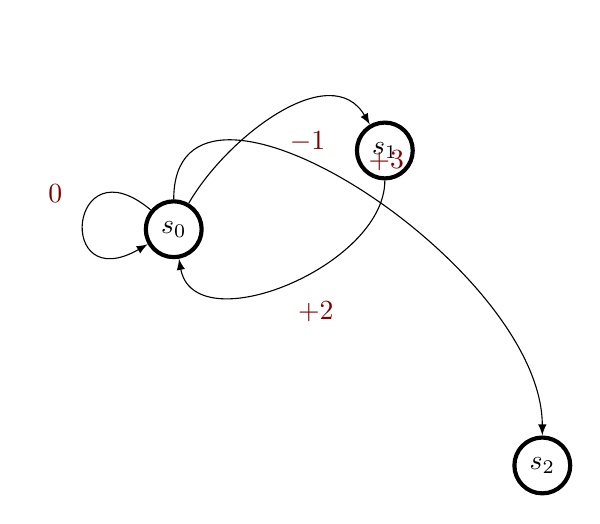
\begin{tikzpicture}[auto,node distance=58mm,>=latex]
    \tikzstyle{round}=[thick,draw=black,circle]
    \node[round] (s0) {$s_0$};
    \node[round, above=10mm, right=23mm] (s1) {$s_1$};
    \node[round, below=30mm, right=43mm] (s2) {$s_2$};

    \draw[->] (s0) [out=60,in=120] to node {} node [swap] {\textcolor{Maroon}{$-1$}} (s1);
    \draw[->] (s1) [out=-90,in=-80] to node {\textcolor{Maroon}{$+2$}} node [swap] {} (s0);
    \draw[->] (s0) [out=90,in=90] to node {\textcolor{Maroon}{$+3$}} node [swap] {} (s2);
    \draw[->] (s0) [out=140,in=210,loop] to node {} node [swap] {\textcolor{Maroon}{$0$}} (s0);




\end{tikzpicture}

\caption{A visual representation of a simple MDP. For each state transition the corresponding reward is presented in red.}
\label{fig:mdp}
\end{figure}

When dealing with MC learning, it can be possible that a certain state is visited more than once before a terminal state is reached. In the MDP represented in Fig. \ref{fig:mdp} this is the case for $s_0$. If that happens, one must decide when to update $V(s)$ and which value to use as $G_t$, as different state visits result in different $G_t$ values. There are two typical ways to deal with this: either update $V(s)$ only once, or one can update $V(s)$ each time the state is visited by simply using as $G_t$ the average of all the different discounted returns. 
While several successful applications of MC methods exist \cite{jaakkola1995reinforcement,liu1998sequential,lazaric2007reinforcement}, a well known issue from this family of algorithms is that they suffer from highly biased updates. In fact, one needs to compute the sum presented in Eq. \ref{eq:goal} over all visited states, resulting in returns with considerable variance. It is easy to see how this can become an issue, especially when the length of the episodes increases. In fact, the larger the episode's length, the more significant the variance of the updates. Furthermore, an additional drawback of MC methods is that one must wait until the agent visits a terminal state before being able to perform an update that is based on Eq. \ref{eq:mc_update}, a drawback that is addressed by the methods that are presented hereafter.   

\subsection{Temporal Difference Learning}
\label{sec:td_learning}
Temporal Difference (TD) Learning \cite{sutton1984temporal,sutton1988learning} is a learning paradigm that allows overcoming the issues mentioned above that characterize MC learning based methods. The key idea of TD-Learning is to update the value of each state with respect to a single MC update, therefore overcoming the hurdle of having to wait for the end of an episode before being able to update the value of a state. Just as MC methods TD-Learning algorithms also learn an optimal value function based on the experience that the agent collects. However, these algorithms base their updates only on the value of a single, consecutive state rather than on the real discounted return that is dependent on the entire sequence of visited states. Updating the value of a state with respect to the value of its successor state only is a technique that comes with the name of \textcolor{RoyalBlue}{bootstrapping}, and is a very effective design choice that reduces the variance in the updates. Bootstrapping can be used to learn the $V$ function and the $Q$ function and is at the core of the most popular model-free RL algorithms. The first and simplest form of TD-Learning was introduced by \citet{sutton1988learning} for learning the state-value function with an algorithm that updates the value of a state based on the following learning rule:
\begin{equation}
	V(s_t):= V(s_t) + \alpha \big[r_t + \gamma V(s_{t+1}) - V(s_t)\big].
	\label{eq:td_learning_v}
\end{equation}
We can now clearly see that differently from what happens in the MC update presented in Eq. \ref{eq:mc_update} the update of a state now only depends on the reward and the value of the next state. This quantity is denoted as the TD-error $\delta_t$ and is defined as:
\begin{equation}
	\delta_t = r_t + \gamma V(s_{t+1}) - V(s_t).
\end{equation}
where $r_t + \gamma V(s_{t+1})$ is also known as the TD-target.
If we again consider the simple MDP represented in Fig. \ref{fig:mdp} and assume that the value of each state of the process is set to $0$ while the discount factor $\gamma$ is this time set to $0.5$ and $\alpha$ is again $0.5$, a TD update for $V(s_0)$ based on a policy resulting in state $s_2$ will result into the new value estimate of $1.5$. 
TD-Learning is a very effective strategy for building algorithms that can learn in an online, fully incremental fashion as one only needs to wait for a single time-step before updating the considered value function. Due to its striking simplicity, TD-Learning has been widely adopted by RL practitioners developing algorithms for learning the $Q$ function. We will present some of the most important algorithms hereafter. 

\paragraph{\textbf{\uppercase{Q}-\uppercase{L}earning}} Introduced by \citet{watkins1992q} is arguably the most popular model-free RL algorithm. It works by keeping track of an estimate of the state-action value function $Q: \mathcal{S} \times \mathcal{A} \rightarrow \Re$ and updates each visited state-action pair with the following update rule:
\begin{equation}
Q(s_t,a_t):=Q(s_t,a_t) + \alpha\big[r_t + \gamma \:\underset{a\in \mathcal{A}}{\max} Q(s_{t+1},a_t) - Q(s_t, a_t) \big].
\label{eq:q_learning}
\end{equation}
The key component of Q-Learning's update rule is the $\max$ operator, which characterizes its TD-error and that is necessary for constructing the TD-target. Since there are as many Q values as there are actions available to the agent, one must choose which Q value to use as a reference when updating the value of the state-action pair that the agent is currently visiting. The $\max$ operator simply chooses the state-action pair with the largest Q value, a simple design choice that has the appealing property of making Q-Learning converge to $Q^{*}(s, a)$ with probability 1 as long as all state-action pairs are visited infinitely often. Interestingly, this guarantee holds even if the agent follows a random policy. The $\max$ operator also defines Q-Learning as an \textcolor{RoyalBlue}{off-policy} learning algorithm, since the Q values chosen for the construction of the TD-target might not correspond to the ones that are associated with the state that the agent will visit after having updated its $Q$ function.

\paragraph{\textbf{\uppercase{SARSA}}} Also known as "online Q-Learning" \cite{rummery1994line} can be seen as the most straightforward extension of the TD-Learning method presented in Eq. \ref{eq:td_learning_v}, and similarly to Q-Learning is an algorithm that aims at learning the state-action value function $Q$. The key idea of SARSA is to update a state-action value with respect to the Q value that is associated to the state that the agent will visit after a certain action is performed. Therefore, SARSA does not use the $\max$ operator within its TD-error and constructs TD-targets that represent the policy that the agent is following, a characteristic that defines SARSA as an \textcolor{RoyalBlue}{on-policy} RL algorithm. The way SARSA learns the $Q$ function is given by the following update rule
\begin{equation}
	Q(s_t,a_t):=Q(s_t,a_t) + \alpha\big[r_t + \gamma Q(s_{t+1},a_{t+1}) - Q(s_t, a_t) \big], 
	\label{eq:sarsa}
\end{equation}
where we can clearly see how the algorithm uses all the elements of the quintuple of events $(s_t, a_t, r_t, s_{t+1}, a_{t+1})$ a property that gives rise to the name $sarsa$. Not using the $\max$ operator in Eq. \ref{eq:sarsa} results in an algorithm that, differently from Q-Learning, does not directly learn the optimal $Q$ function anymore, but rather learns to estimate $Q^{\pi}(s,a)$. This has the drawback of not guaranteeing convergence to $Q^{*}(s,a)$ for any random policy anymore. To overcome this, SARSA needs an exploration policy that is greedy in the limit of infinite exploration \cite{singh2000convergence}. This can be achieved with the popular $\epsilon$-$\text{greedy}$ selection policy which defines the action that the agent takes as:
\begin{equation}
a_t = \begin{cases}
\underset{a\in\mathcal{A}}{\argmax} \ Q(s_t,a) &\text{with probability $1-\epsilon$}\\
a \sim \mathcal{U}(\mathcal{A}) &\text{with probability $\epsilon$}
\end{cases}
\label{eq:e_greedy}
\end{equation}
where $\epsilon$ is a hyperparameter that changes while training progresses. During early training iterations, its value is close to $1$, while it approaches $0$ by the end of training. This allows the agent to take actions that are representative of a large set of policies when the learned $Q$ function does not yet correspond to $Q^{*}(s,a)$, while it will favor greedy actions at the end of training. This is a simple, yet effective strategy that deals with the \textcolor{RoyalBlue}{exploration-exploitation} dilemma. It is however worth noting that its use is not limited to on-policy RL algorithms only. Furthermore, the method presented in Eq. \ref{eq:e_greedy} represents only one possible way of balancing exploration and exploitation, and although it is arguably the most popular of such methods, it is not the only existing one. We refer the reader to chapter 5 of \cite{wiering1999explorations} for a thorough analysis of different exploration algorithms.

\paragraph{\textbf{\uppercase{D}ouble \uppercase{Q}-\uppercase{L}earning}} In some environments, Q-Learning is known to perform poorly. This poor performance stems from the fact that the algorithm largely overestimates some state-action values due to the $\max$ operator in its TD-error \cite{thrun1993issues}. The $\max$ operator serves for constructing an approximation of the maximum expected action-value of a state, which, as discussed by \citet{hasselt2010double}, is a technique that results in positively biased estimates \cite{van2004rational,smith2006optimizer}. In some RL problems, this can significantly influence the learning process, which has led the RL community to develop a set of solutions that try to mitigate this bias \cite{lee2013bias,lee2019bias,zhu2020self,pentaliotis2021variation}. Among the different solutions, Double Q-Learning \cite{hasselt2010double} is probably the most popular one. Its main idea is to keep track of two different state-action value functions, $Q_1$ and $Q_2$, which get alternatively used for selecting which action to perform. When one of the two $Q$ functions determines the action that maximizes the state-action value of the next state, the remaining value function is used for evaluating this estimate. This can be achieved with the following rule:
\begin{equation}
	Q_1(s_t,a_t):=Q_1(s_t,a_t) + \alpha\big[r_t + \gamma \: Q_2(s_{t+1},a^{*}) - Q_1(s_t, a_t) \big],
\label{eq:double_q_learning}
\end{equation}
where $a^{*}=\argmax_{a\in \mathcal{A}} Q_1(s_{t+1},a)$. Note that at each time step, only one of the two $Q$ functions gets updated. While training progresses, the choice of which $Q$ function to update is determined randomly. In the case it is $Q_2$, the update rule is identical to the one presented in Eq. \ref{eq:double_q_learning} with the only difference being that the role of the two $Q$ functions is swapped. Double Q-Learning converges to the optimal state-action value function with probability $1$ under the same conditions as Q-Learning. \citet{hasselt2010double} shows that using two separate $Q$ functions significantly mitigates the overestimation bias. Yet, this comes at the price of an algorithm that is twice more expensive in terms of memory requirements. It is also worth noting that although Double Q-Learning does not overestimate the state-action values, it might instead underestimate them, which in some environments can still yield poor performance.


\paragraph{\textbf{\uppercase{QV}($\lambda$)-\uppercase{L}earning}} First introduced by \citet{wiering2005qv} and further developed by \citet{wiering2009qv} is an on-policy RL algorithm which differently from the previously introduced methods keeps track of an estimate of the state-value function $V:\mathcal{S}\rightarrow\mathbb{R}$ alongside the usual estimate of the state-action value function $Q:\mathcal{S}\times\mathcal{A}\rightarrow\mathbb{R}$. Since the goal is to jointly learn two value functions, QV($\lambda$)-Learning requires two separate update rules. The $V$ function is learned via the same form of TD-Learning that we introduced in Eq. \ref{eq:td_learning_v}, with the only difference being the addition of the eligibility traces $e_t(s)$ at the end of the update rule (an RL technique that we will review in Chapter \ref{ch:dqv_family_of_algorithms}). QV($\lambda$)-Learning, therefore, learns the $V$ function with the following update rule:
\begin{equation}
V(s):= V(s) + \alpha \big[ r_{t} + \gamma V(s_{t+1}) - V(s_t) \big] e_{t}(s).
\label{eqch02:qv_lambda_v_update}
\end{equation}
Since as discussed earlier only learning the $V$ function is not sufficient for deriving an optimal policy one needs to learn the $Q$ function as well. In QV($\lambda$)-Learning this is done as follows:
\begin{equation}
Q(s_{t}, a_{t}):= Q(s_{t}, a_{t}) + \alpha \big[r_{t} + \gamma V(s_{t+1}) - Q(s_{t}, a_{t}) \big].
\label{eqch02:qv_lambda_q_update}
\end{equation}
An attractive property of the algorithm is that it uses the same TD-target ($r_t + \gamma V(s_{t+1})$) for defining the two different TD-errors that are required for learning the state-value and the state-action value functions. Among the main insights that motivate learning two value functions over one, \citet{wiering2005qv} mentions the possibility that the $V$ function, since it does not depend on the agent's actions, might converge faster than the $Q$ function. As described earlier, the $V$ function only depends on the state space of the MDP, which by definition is smaller than the state-action space. For a more in-depth and formal presentation of the conditions that show the benefits of jointly learning the $V$ function alongside the $Q$ function, we refer the reader to chapter 5 of \cite{van2011insights}.


\section{Function Approximators}
\label{sec:function_approximators}
If it is true that model-free RL algorithms are very powerful methods for learning an optimal policy when parts of the MDP are unknown, it is also true that all the algorithms mentioned above suffer from the \textcolor{RoyalBlue}{curse of dimensionality}. Model-free algorithms are typically implemented in a tabular fashion, meaning that the state values, or state-action values, are stored within tables of sizes $|\mathcal{S}|$ and $|\mathcal{S}\times\mathcal{A}|$ respectively. Albeit straightforward and easy to implement, such an approach presents severe limitations. The first major drawback of the tabular representation approach is that it does not scale well with respect to the MDP complexity. If the environment state and action spaces become very large, storing a table quickly becomes unfeasible in terms of storage space. Furthermore, tabular representations are also unable to deal with continuous states. A natural solution to this problem could consist in discretizing the state space; however, this approach still results in the aforementioned storage space issues when done thoroughly. Therefore, if one wants to use RL techniques, even when the state space of the MDP is large, a better solution is needed. This solution is based on \textcolor{RoyalBlue}{parametrized function approximation}. In this context, the goal is not to learn the exact value function anymore but to rather replace its tabular representation with a parametrized function. This function parameters can then be adjusted based on the RL algorithms that we introduced in Sec. \ref{sec:td_learning}. 

\subsection{Linear Functions}
\label{sec:linear_functions}

The most straightforward type of function approximator one can use is a linear function. Given a state-action tuple that gets represented as a feature vector $\vec{x}(s)=[x_1(s), x_2(s), ..., x_q(s)] \in \mathds{R}^q$, and a function parametrized by a vector of parameters $\mathbold{\theta}^a\in\mathds{R}^q$ for each action $a\in\mathcal{A}$, as shown in \cite{wiering2004convergence}, we can redefine the value of a state-action pair as:
\begin{equation}
	Q(s,a) = \sum_i \theta^a_{i} x_i(s).
\end{equation}
Given a trajectory $\langle s_t,a_t,r_t,s_{t+1}\rangle$, the Q-Learning algorithm presented in Eq. \ref{eq:q_learning} can now be used for updating the parameters $\theta^a_i$ for all $i$ with the following update rule:
\begin{equation}
	\theta^{a_t}_{i} := \theta^{a_t}_{i} + \alpha(r_t +\gamma\:\underset{a\in \mathcal{A}}{\max} Q(s_{t+1},a_t) - Q(s_t, a_t)) x_i(s_t).
	\label{eq:q_learning_fa}
\end{equation}
We can observe that this update rule modifies the parameter vectors $\mathbold{\theta}^a$ by minimizing the mean squared error loss between a given state-action tuple and Q-Learning's TD-target since  
\begin{equation}
\begin{split}
	& \mathcal{L}(\theta) = \frac{1}{2}\big(y_t - Q(s_t, a_t)\big)^2 \mbox{ with } y_t = r_t +\gamma\:\underset{a\in \mathcal{A}}{\max} Q(s_{t+1},a_t) \\ 
	& \frac{\partial\mathcal{L}}{\partial \theta_{i,a_t}}=-\big(y_t - Q(s_t, a_t)\big) x_i(s_t)  \\ 
 	& \theta^{a_t}_{i} := \theta^{a_t}_{i} + \alpha(r_t +\gamma\:\underset{a\in \mathcal{A}}{\max} Q(s_{t+1},a_t) - Q(s_t, a_t)) x_i(s_t).
\end{split}
\end{equation}

Similar steps can be used for adapting all of the RL algorithms that we introduced in the previous section. As a representative example for the on-policy learning case let us consider the SARSA algorithm. One can learn an approximation of the $Q$ function by updating the parameters of a linear function as follows:

\begin{equation}
	\theta^{a_t}_{i} := \theta^{a_t}_{i} + \alpha(r_t +\gamma Q(s_{t+1},a_{t+1}) - Q(s_t, a_t)) x_i(s_t).
\end{equation}
Linear functions can yield successful results \cite{lane1992theory, park1993approximation, mcculloch1943logical} as they can indeed deal with the aforementioned curse of dimensionality problem. However, \textcolor{RoyalBlue}{non-linear} functions are usually preferred since their representational power is even larger than the one of linear methods. Throughout this dissertation, we are interested in non-linear functions that come in the form of deep neural networks. As we have seen in the previous chapter, neural networks such as e.g convolutional networks are able to learn very rich representations from their inputs. However, this also makes these kinds of models particularly challenging to train in an RL context. We will now describe how one can successfully deal with some of the challenges that characterize the use of deep neural networks in RL by presenting some of the most important algorithms that have been introduced over the years.    

\section{Deep Reinforcement Learning}
\label{sec:deep_reinforcement_learning}
Before looking into how RL algorithms should be integrated within deep neural networks, it is important to mention that RL techniques have been successfully combined with (less powerful) neural networks for over three decades. In fact, the field known as \textcolor{RoyalBlue}{Connectionist Reinforcement Learning} (CRL) resulted in the very first algorithms that managed to outperform human experts on specific tasks. Among the multiple possible examples of this family of techniques, we mention the TD-Gammon program introduced by \citet{tesauro1994td}. TD-Gammon successfully learns an approximation of the popular Backgammon boardgame's evaluation function through the same TD-Learning methods that we presented in Sec. \ref{sec:td_learning}. Tesauro's program achieved a level of play comparable to the one of the top human Backgammon players of its time and is even nowadays considered one of the most important RL breakthroughs. For a more detailed presentation about the successful applications of CRL algorithms, we refer the reader to \cite{bucsoniu2011approximate}.  

While certainly successful for a certain set of problems (see for example chapter $1$ of \cite{sabatelli2017learning}), CRL techniques also present severe limitations. Since they only use multi-layer perceptrons as function approximators, these algorithms cannot be used for tackling problems where the state representation of the MDP is highly dimensional. To overcome this, more complicated and powerful networks are required. \textcolor{RoyalBlue}{Deep Reinforcement Learning} (DRL) \cite{arulkumaran2017deep, li2017deep, franccois2018introduction} is a research field that combines RL algorithms with deeper and more complex neural architectures. In value based model-free DRL we are interested in learning an approximation of either the optimal state-value function $V(s;\theta)\approx V^{*}(s)$ or the optimal state-action value function $ Q(s,a;\theta)\approx Q^{*}(s,a)$ with a deep neural network that comes with parameters $\theta$
and that usually comes in the form of a convolutional neural network. We now describe some of the algorithms which have contributed to the development of DRL the most. 

\paragraph{\textbf{\uppercase{D}eep \uppercase{Q}-\uppercase{L}earning (\uppercase{DQN})}} Just like Q-Learning is arguably the most important tabular model-free RL algorithm, so is DQN when it comes to DRL. First introduced by \citet{mnih2013playing} and then made popular by the work presented in \cite{mnih2015human} this algorithm can certainly be considered as the very first successful example of a neural network that is able to learn an approximation of the optimal state-action value function just from high sensory inputs (in this case images). As the name suggests, Deep Q-Learning (DQN)\footnote{In DQN the `N" in the acronym stays for `Network" and replaces what could have been the, arguably more intuitive, `L" of Learning.} is based upon the Q-Learning algorithm and aims at learning an approximation of the optimal state-action value function $Q$. This is done by reshaping Q-Learning's update rule, presented in Eq. \ref{eq:q_learning}, into a differentiable loss function that can be used for training a convolutional network. This is achieved through the following objective function:
\begin{multline}
	\mathcal{L}(\theta) = \mathds{E}_{\langle s_{t},a_{t},r_{t},s_{t+1}\rangle\sim U(D)} \bigg[\big(r_{t} + \gamma \: \underset{a\in \mathcal{A}}{\max}\: Q(s_{t+1}, a; \theta^{-}) \\ - Q(s_{t}, a_{t}; \theta)\big)^{2}\bigg].
\label{eq:dqn}
\end{multline}

We can start by observing that the general principles that characterize the algorithm are the same ones that made it possible to generalize Q-Learning to the use of linear function approximators, however, differently from when a linear function is used, the mapping between input and feature spaces is now naturally not preserved anymore. Similarly to what we presented in Sec. \ref{sec:linear_functions}, we can see from Eq. \ref{eq:dqn} that learning $Q(s,a,\theta)$ is again achieved by minimizing the squared error loss between the $Q(s_t,a_t;\theta)$ estimates and the off-policy TD-target
\begin{equation}
    y^{DQN}_{t} = r_{t} + \gamma \: \underset{a\in \mathcal{A}}{\max}\: Q(s_{t+1}, a; \theta^{-}).
\label{eq:dqn_td}
\end{equation}
Despite this similarity, DQN requires some additional algorithmic design choices, without which it would turn out to be almost impossible to successfully train a neural network with Eq. \ref{eq:dqn}. These additions, which significantly make DQN differ from the algorithm presented in Eq. \ref{eq:q_learning_fa} are the following:
\begin{itemize}
	\item \textcolor{RoyalBlue}{Experience Replay}: a memory buffer, $D$, represented as a queue which stores RL trajectories of the form $\langle s_{t}$, $a_{t}$, $r_{t}$, $s_{t+1} \rangle$. Once this memory buffer is filled with a large set of these quadruples, DQN uniformly samples batches of trajectories for training its network. This makes it possible to exploit past trajectories multiple times by reusing them while training, which makes the overall algorithm more sample efficient. Furthermore, using a memory buffer also improves the stability of the training procedure. Recall that each trajectory is representative of a certain episode. By repeatedly randomly sampling a different $\tau$ from the memory buffer, a resulting mini-batch of trajectories will be representative of different episodes and of different policies. As a consequence, the correlation between trajectories within a mini-batch will be small. Although made popular by the DQN algorithm, using an experience replay buffer for tackling sequential decision making problems was already presented by \citet{lin1992self}.
		
	\item \textcolor{RoyalBlue}{Target Network}: We can observe from Eq. \ref{eq:dqn_td} that the TD-target used by DQN for bootstrapping is not computed by the $Q$ network that is being optimized ($\theta$), but rather from a second separate network that is parametrized with $\theta^{-}$. This second network has the same structure as the main $Q$ network, but its weights do not change each time RL experiences are sampled from $D$. On the contrary, its weights are temporally frozen and only periodically get updated with the parameters of the main network $\theta$ as defined by an appropriate hyperparameter. Note that this is a design choice that is not motivated by the TD-Learning paradigm that we presented in Sec. \ref{sec:td_learning}, where we have seen that TD-Learning based methods learn in a fully online fashion by updating their value estimates based on their own future estimates. With a target-network, although the $\theta$ network still learns via the methods of temporal differences, it now requires an auxiliary, external model if it wants to successfully learn $\approx Q^{*}(s,a;\theta)$. Several works have studied the target network's role to understand why this design choice appears to be necessary for DRL. Yet, the DRL community does not fully understand the role of $\theta^{-}$. For more about this topic, we refer the reader to \cite{kim2019deepmellow, piche2021beyond}.

\end{itemize}

With all these concepts in place we can show that given a training iteration $i$, differentiating this objective function with respect to $\theta$ gives the following gradient: 
\begin{multline}
\nabla_{\theta_{i}} \mathcal{L}(\theta_{i}) = \mathds{E}_{\langle s_{t},a_{t},r_{t},s_{t+1}\rangle\sim U(D)} \bigg[\big(r_{t} + \\ \gamma \: \underset{a\in \mathcal{A}}{\max}\: Q(s_{t+1}, a; \theta^{-}_{i-1})  - Q(s_{t}, a_{t}; \theta_{i})\big)\nabla_{\theta_{i}} Q(s_{t}, a_{t}; \theta_{i})\bigg].
\label{eq:dqn_gradient}
\end{multline}

The DQN algorithm showcased its entire potential in \cite{mnih2015human} where Mnih and colleagues developed a convolutional neural network that trained with Eq. \ref{eq:dqn} learned how to successfully play most of the \texttt{Atari} games that are part of the popular Atari Arcade Learning Environment (ALE) \cite{bellemare2013arcade}, a well-known platform that even nowadays serves as a benchmark for testing the performance of DRL algorithms. In the ALE, a DRL algorithm has to learn how to play $57$ different emulations of \texttt{Atari} games which are specifically designed within a simulator (see Fig. \ref{fig:atari_games} for a visualization of some of the games that are part of the ALE suite). Remarkably, DQN not only learned how to play most of the games of the platform but also achieved a final performance that, on most games, was superior to the one of human expert players. What is even more remarkable is that this was achieved by providing as inputs to the network the images representing the game only, therefore making the model learn just from its own experience in a pure model-free RL fashion. Since then, DQN has been successfully used for a large variety of applications ranging from healthcare \cite{tseng2017deep,raghu2017continuous}, robotics \cite{kalashnikov2018qt} and natural language processing \cite{he2015deep, narasimhan2015language} to even particle physics \cite{liu2017learning, sajedian2020design}. However, despite all these remarkable applications, the algorithm still comes with some drawbacks, some of which are addressed by the algorithms presented below.

\begin{figure}[ht!]
\centering
  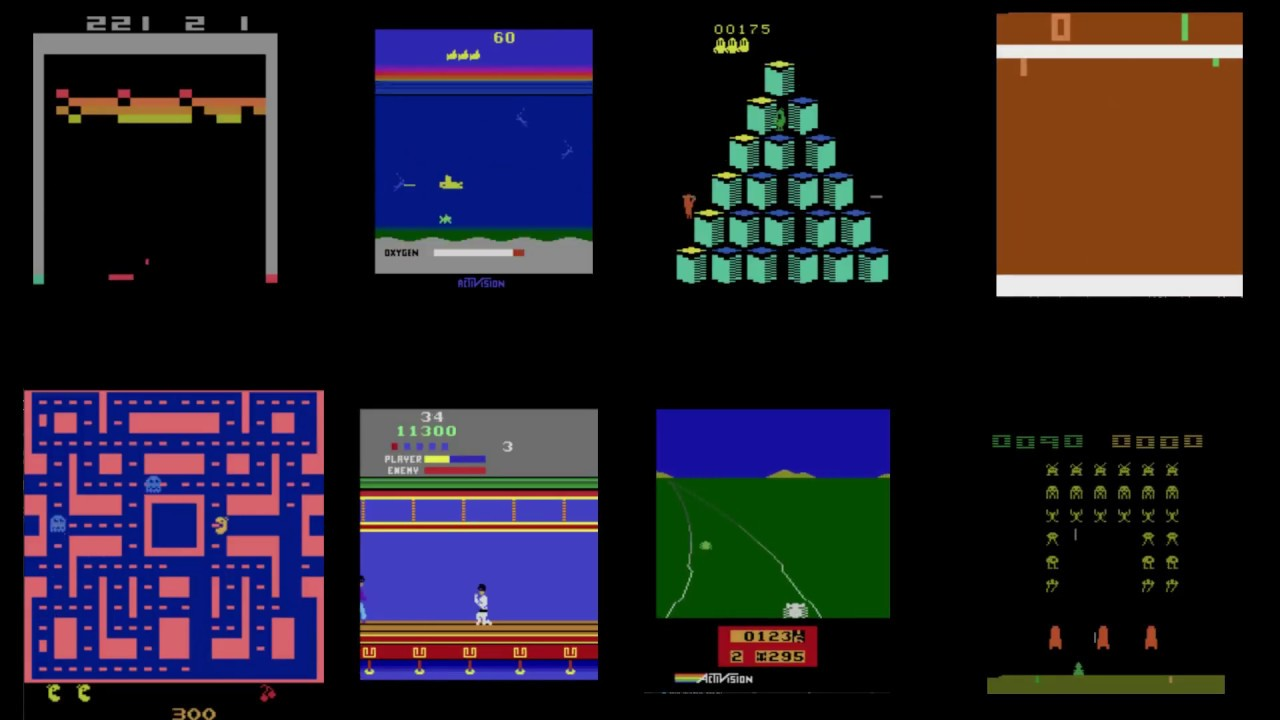
\includegraphics[width=10cm]{./Images/Chapter02/atari_games}
  \caption{A visual representation of some of the \texttt{Atari} games that are part of the Arcade Learning Environment (ALE) \cite{bellemare2013arcade}. From left to right \texttt{Breakout, Seaquest, Qbert, Pong, MsPacman, KungFu-Master, Enduro} and \texttt{Space Invaders}. Most of these games will be of interest in Chapter \ref{ch:dqv_family_of_algorithms} and Chapter \ref{ch:dqn_transfer}.}
  \label{fig:atari_games}
\end{figure}


\paragraph{\textbf{\uppercase{D}ouble \uppercase{D}eep \uppercase{Q}-\uppercase{L}earning (\uppercase{DDQN})}} \citet{van2016deep} showed that the DQN algorithm suffers from the same issue that also characterizes the Q-Learning algorithm: the overestimation bias of the $Q$ function. They show that DQN is prone to learn overestimated Q-values because the same values are used both for selecting an action ($\underset{a\in \mathcal{A}}{\max}$) as well as for evaluating it ($Q(s_{t+1},a;\theta^{-})$). This becomes clearer when re-writing DQN's TD-target presented in Eq. \ref{eq:dqn_td} as:
\begin{equation}
    y^{DQN}_{t} = r_{t} + \gamma \: Q(s_{t+1}, \underset{a\in \mathcal{A}}{\argmax}\: Q(s_{t+1}, a; \theta); \theta^{-}). 
\end{equation}{}
As a result, DQN tends to approximate the expected maximum value of a state, instead of its maximum expected value. As presented in Sec. \ref{sec:td_learning}, in the tabular case this can be solved by keeping track of two separate $Q$ functions, and by randomly preferring one $Q$ function over the other when it comes to selecting which action to execute. DDQN generalizes this idea and untangles the action selection process from its evaluation by taking advantage of the previously introduced target network $\theta^{-}$. DDQN's target stays the same as in DQN with the main difference being that the selection of an action, given by the online Q-network $\theta$, and the evaluation of the resulting policy, given by $\theta^{-}$, can now result into smaller overestimations simply by symmetrically updating the two sets of weights ($\theta$ and $\theta^{-}$) which can easily be achieved by regularly switching their roles during training. While not always significantly impacting the performance of DQN (one can still act optimally even if some actions are associated to unrealistically high $Q(s,a)$ estimates), there are also cases for which the overestimation bias of the $Q$ function significantly slows down the training process, and even prevents the DQN algorithm from improving its policy over time at all. We will come back to this issue in Chapter \ref{ch:dqv_family_of_algorithms}. 


\paragraph{\textbf{\uppercase{P}rioritized \uppercase{E}xperience \uppercase{R}eplay (\uppercase{PER})}} We have seen that next to the target network $\theta^{-}$ an equally important role within the DQN algorithm is played by the experience replay memory buffer $D$. \citet{schaul2015prioritized} showed that the efficiency of how Deep Q-Networks use this buffer could be improved. Their claim stems from the fact that, as shown in Eq. \ref{eq:dqn}, the RL trajectories that get sampled from the memory buffer when constructing a mini-batch of trajectories are sampled uniformly ($\sim U(D)$). This approach has the main drawback that it considers each $\tau$ stored in the buffer as equally important and representative for training. However, it is easy to imagine learning situations where some trajectories are more valuable than others. For example, at the beginning of training, most of the trajectories contained within $D$ will be representative of early agent-environment interactions. It is, therefore, safe to assume that the network will learn the $Q(s,a)$ estimates representative of these early dynamics much faster than it will learn the $Q$ values that are associated with trajectories occurring more rarely. The idea of PER is to use only highly informative trajectories when it comes to building the mini-batches that are used for training the network. The importance of different trajectories is given by their respective TD-error. PER ensures that the probability of sampling trajectories is proportional to their respective TD-errors: the higher the TD-error, the larger the probability for a specific $\tau$ to be sampled. In practice, given a trajectory $\tau$, the probability of sampling it is given by the following equation:
\begin{equation}
	P(\tau)=\frac{p_{\tau}^{\alpha}}{\sum_k p_{k}^{\alpha}}
\end{equation}
where $p_{\tau}$ is $|\delta_\tau + \epsilon|$ with $\epsilon$ being a small positive number ensuring that the probability of sampling a trajectory remains positive even in the edge case where the TD-error is $0$. Although simple and intuitive, implementing a PER buffer is not that straightforward and still presents some algorithmic caveats that need to be taken into account. Yet, if done correctly it dramatically improves the sample efficiency of Deep Q-Networks \cite{narasimhan2015language}.

\paragraph{\textbf{\uppercase{D}ueling \uppercase{N}etworks}} While the DDQN algorithm directly tackles a fundamental algorithmic bias that characterizes the way DQN learns the $Q$ function, and PER addresses the inefficiency of its memory buffer, the contribution presented by \citet{wang2016dueling} is of slightly different nature. Their work consists of a novel type of neural architecture called the Dueling Network. This is a contribution that resembles more the kind of progress that is made by the supervised learning community, which, as we discussed in the previous chapter, has put a lot of effort into developing novel neural architectures for tackling computer vision tasks. Nevertheless, Wang's work is a perfect example that showcases how in DRL, carefully designing the function approximator is just as important as properly defining its objective function. A Dueling network is a network that, after performing a series of convolutions, instead of directly outputting the state-action values for a specific state as DQN and DDQN do, adds some intermediate computations. The idea is to estimate the value of a state and the advantages for each action before outputting the final $Q$ values. The state values are computed based on Eq. \ref{eq:state_value_function}, while the advantage function $A$ is simply the difference between the $Q$ function and the $V$ function:
\begin{equation}
	A^{\pi}(s,a) = Q^{\pi}(s,a) - V^{\pi}(s).
\end{equation}
To successfully estimate state values, advantages, and state-action values, the network requires a specific architecture consisting of three separate streams. Each stream is responsible for estimating one of the three value functions and is initialized with its own parameters $\theta^{(\cdot)}$. The final $Q$ function of the model is then obtained by combining what is learned by each stream as follows:
\begin{multline}
	Q(s,a;\theta^{(1)},\theta^{(2)},\theta^{(3)}) = V\bigl(s;\theta^{(1)},\theta^{(3)}\bigr) + \\
	\bigl(A(s,a;\theta^{(1)},\theta^{(2)}) - \underset{a_{t+1}\in \mathcal{A}}{\max}\: A(s, a_{t+1};\theta^{(1)},\theta^{(2)}) \bigr).
	\label{eq:dueling}
\end{multline}
Building a network with different task-specific streams is a design choice that resembles the way models are built when tackling multitask classification tasks. However, note that the output of each stream that either estimates the state values or the advantage function gets aggregated in a final layer that estimates the state-action values. Training a Dueling Network is done by minimizing the same objective function that is also minimized by DQN and DDQN. The idea of taking into account the $V$ function when learning the $Q$ function is a concept which will come back, in a different flavor, in Chapter \ref{ch:dqv_family_of_algorithms} and Chapter \ref{ch:dqn_transfer}.

\paragraph{\textbf{\uppercase{P}olicy \uppercase{G}radient \uppercase{M}ethods}} So far we have only considered algorithms that are part of the action-value family of methods, which, as explained in Sec. \ref{sec:learning_value_functions} are techniques that derive an optimal policy from a learned $Q$ function. Yet, there is a collection of algorithms that is able to learn a policy directly, and that therefore bypasses the requirement of having to consult state-action values when it comes to action selection. These methods, which have contributed to the development of DRL just as much as action-value methods, come with the name of Policy Gradients. They directly parametrize a policy at each time-step as $\pi(a|s;\theta)=\text{Pr}\:\{a_t = a| s_t=s;\theta_t=\theta\}$ and seek to optimize the parameters $\theta$ such that the performance of the policy is maximized. Note that this is drastically different from all the methods which we have seen so far, where the aim, in fact, was to minimize the TD-error through gradient descent optimization. Since policy gradients aim to maximize their performance, they learn via gradient ascent and therefore update their parameters as follows
\begin{equation}
	\theta \leftarrow \theta + \alpha \nabla \xi(\theta).
\end{equation}
Here $\alpha$ is again the learning rate, and $\xi$ is a measure that quantifies the performance of the policy. Similarly to action-value based methods, one can parametrize a policy either with a linear function or with a deep neural network. When the action space is discrete, it is common practice to parametrize $\pi$ through the same exponential softmax distribution, which we have seen in the previous chapter when presenting neural networks trained for classification tasks. Therefore we have
\begin{equation}
	\pi(a|s;\theta) = \frac{e^{h(s,a;\theta)}}{\sum_b e^{h(s,b;\theta)}}
\end{equation}
where $h(s,a;\theta)$ is any function approximator. By doing so, policy gradient methods naturally deal with the exploration-exploitation trade-off since they simply assign different probabilities to different actions. This also allows these methods to approach a deterministic policy (which cannot be achieved when using $\epsilon$-greedy action selection) and makes these algorithms arguably easier to train since learning a policy could be easier than learning state-action returns. The fundamental result which allows optimizing any differentiable policy is the policy gradient theorem \cite{sutton1999policy}. \citet{sutton1999policy} show that the gradient of $\pi$ does not depend on the gradient of the state distribution and that it can therefore be expressed as follows:
\begin{equation}
	\nabla \xi(\theta) = \sum_{s} \mu(s) \sum_{a} Q^{\pi}(s,a) \nabla \pi(a|s;\theta)
\end{equation}
where $\mu(s)$ is the stationary on-policy distribution under $\pi$. By expressing the gradient as such, it is now possible to optimize $\pi$ even when the state distribution of the environment is unknown (as discussed in Sec. \ref{sec:learning_value_functions}). Policy gradient methods can be used for learning a policy through the same kind of techniques which in Sec. \ref{sec:learning_value_functions} were used for learning value functions. Within the Monte Carlo setting the arguably most important of such algorithms is REINFORCE \cite{williams1992simple}, while Actor-Critic algorithms \cite{lillicrap2015continuous,schulman2015high,schulman2015trust,wang2016sample,mnih2016asynchronous,schulman2017proximal,haarnoja2018soft,fujimoto2018addressing} learn a policy with the additional help of a bootstrapped value function (typically $V$ or $A$).


\paragraph{\textbf{\uppercase{R}ainbow}} From the examples above, it is clear that much progress has been achieved by the DRL community in creating algorithms capable of learning faster and better. Explaining all the individual value-based contributions that have made DRL the popular research field it is nowadays \cite{henderson2018deep}, is beyond the scope of this chapter. Yet, if there is one algorithm that encapsulates most of the progress that the DRL community has achieved over the last years, that is Rainbow \cite{hessel2018rainbow}. Rainbow is a single, almighty agent that integrates most of the important breakthroughs that DRL researchers have introduced over the last decade within the same algorithm, ranging from the previously mentioned DDQN algorithm and PER system to more recent techniques such as distributional DRL \cite{bellemare2017distributional}, multi-step learning, distributed training \cite{mnih2016asynchronous} and noisy networks \cite{fortunato2017noisy} that allow for better exploration.


\section{The Deadly Triad of Deep Reinforcement Learning}
\label{sec:challenges}
We now end this chapter by presenting one of the main limitations that currently characterizes the field of DRL and that has inspired part of the research that is presented in this dissertation.

The combination of RL with function approximation can result in unstable training and algorithms prone to diverge while learning. As a representative example of what it means for an RL algorithm to diverge, let us consider the following MDP firstly introduced by \citet{tsitsiklis1997analysis}. The MDP consists of three states $s_0, s_1$ and the terminal state $s_2$. Each state is described by a single scalar feature $\psi$ such that $\psi(s_0)=1$, $\psi(s_1)=2$, and $\psi(s_2)=3$. The estimated state-value of each state is therefore given by $V(s)=\psi(s) \cdot w$, where $w$ is the single weight we would like to update. The MDP is represented in Fig \ref{fig:deadly_triad}.  
\begin{figure}[ht!]
	\centering
	\tikzset{
    ->, 
    level distance = 22em,
    minimum size=2em,
    %edge from parent/.style={draw,thick},
    level 1/.style={sibling distance=6em},
    level 2/.style={sibling distance=3em},
    thick/.style = {line width=1.5pt},
    extra thick/.style = {line width=3.5pt},
    red node/.style={shape=circle,draw=red,fill=red!40,thick,inner sep=1.2},
    blue node/.style={shape=circle,draw=blue,fill=blue!40,thick,inner sep=1.2}
}

\tikzstyle{round}=[thick,draw=black,circle]

\begin{tikzpicture}[auto,node distance=58mm,>=latex]
    \tikzstyle{round}=[thick,draw=black,circle]
    \node[round, label=below:$s_0$] (s0) {$w$};
    \node[round, label=below:$s_1$, above=10mm, right=23mm] (s1) {$2w$};
    \node[round, label=below:$s_2$, below=30mm, right=43mm] (s2);

    \draw (s0) -> (s1);
    \draw [->] (s1.90) arc (0:264:4mm); 
    \draw (s1) -> (s2);

    \path [line] (s1.90) -- node [text width=1.5cm,midway,above,align=center] {$1-\epsilon$} arc (0:264:4mm);

    \path [line] (s1) -- node [text width=2.5cm,midway,above,align=center ] {$\epsilon$} (s2);

\end{tikzpicture}

\caption{A visual representation of the MDP proposed by \citet{tsitsiklis1997analysis} that shows how RL algorithms combined with function approximators can diverge.}
\label{fig:deadly_triad}
\end{figure}
Each state transition is associated with a reward of $0$, which means that the optimal weight value for having perfect value predictions is $w^{*}=0$. Let us now assume that we are updating the state-value function based on an on-policy learning scheme as discussed in Sec. \ref{sec:td_learning}. We then know that each time we are updating the state-value function for $s_0$, the value of $s_1$ will, in expectation, also be updated multiple times. This however, changes if we are following an off-policy learning scheme since each time we update the state-value function for $s_0$, we do not necessarily update the value of $s_1$ anymore. As shown by \citet{van2018deep_triad} if we would now update $w$ based on Eq. \ref{eq:td_learning_v} we would have to modify $w$ as $\Delta w \propto r_t +\gamma(V(s_{t+1})-V(s_t))$. Which results into $0+\gamma 2w-w=\gamma 2w-w=(2\gamma-1)w$. If we then set the discount factor $\gamma>0.5$ as is common practice, we can see that we have $2\gamma>1$, which will make any weight $w\neq0$  be updated away from the desired value of $0$. \citet{sutton2018reinforcement} show that the cause of this type of divergence occurs when RL algorithms are combined with three concepts which we have already encountered in this chapter. These concepts are: bootstrapping (Sec. \ref{sec:td_learning}), off-policy learning (Sec. \ref{sec:td_learning}) and function approximation (Sec. \ref{sec:function_approximators}).
This combination is known as the `Deadly Triad" of DRL, and it is well known that if all of these three elements are combined within the same algorithm, divergence can appear. Divergence results in algorithms that are extremely slow to train, or even in agents that are not able to improve their policy over time at all. Throughout this dissertation we will tackle the problem of the Deadly Triad by first introducing novel algorithms that are less prone to diverge (Chapter \ref{ch:dqv_family_of_algorithms}), while in a second approach by investigating whether the particularly long training times that characterize such algorithms can be reduced by adapting transfer learning strategies (Chapter \ref{ch:dqn_transfer}).   




